
\chapter{Introduction} 
\label{ch:Chapter1}
\vfill \newpage
\noindent

PostChat is an innovative Android application that aims to bring back the charm of postcards and bridge the gap between the older and younger generations through the use of modern technology. The app serves as a client-server platform that enables users to create, personalize, and send digital postcards to their loved ones, fostering meaningful connections in today's digital age.
Figure~\ref{fig:OV} illustrates PostChat's use case.

\begin{figure}[!ht]
	\centering
	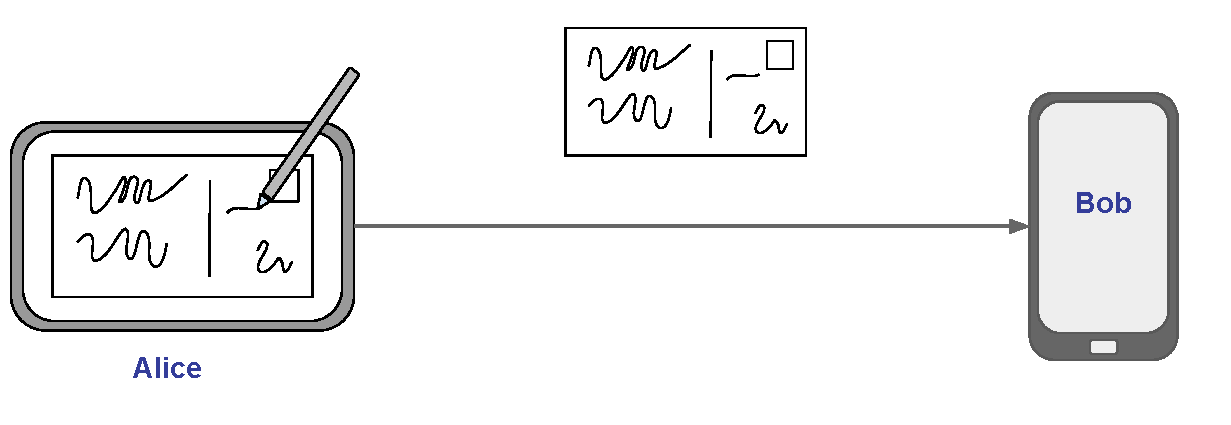
\includegraphics[width=0.75\textwidth]{./Chapter1/Figures/Overview}
	\caption{Overview}
	\label{fig:OV}
\end{figure}

In today's fast-paced world, people have become increasingly reliant on technology to communicate with their friends and family. However, the traditional art of sending postcards has lost its appeal over the years, particularly among the younger generation. With PostChat, we strive to revive this age-old practice and make it relevant again, while also making it accessible and convenient to use for everyone.

The PostChat application operates on a client-server architecture, where the Android app serves as the client and a web API functions as the server. This design allows for seamless communication between users and the server, enabling the creation and transmission of digital postcards with ease.

The PostChat app is meticulously designed to cater to the needs of all age groups, with a user-friendly interface that is easy to navigate. Users have access to a diverse range of postcard templates, allowing them to personalize their messages and express their creativity. Additionally, the app integrates advanced features, such as AI tools tailored for the visually impaired, ensuring an inclusive and empowering experience for all users.

Furthermore, PostChat goes beyond the confines of traditional postcards, as it facilitates real-time communication and community building. Users can create chat groups within the app, enabling them to engage in conversations and share postcards with multiple recipients simultaneously. This feature encourages meaningful interactions and strengthens connections among friends and family.

This report aims to delve deeper into the workings of the PostChat application, analyzing its features, design, usability, and the integration between the Android app and the web API server. The report is organized like this:
\begin{itemize}
	\item Requirements - What has to be done in order to implement this project;
	\item Web Api - The server side application;
	\item HTR Model - Our approach to a HTR model it's limitations and challenges;
	\item Client - The Android client application;	
\end{itemize}